\documentclass{mc2015}

%%%%%%%%%%%%%%%%%%%%%%%%%%%%%%%%%%%%%%%%%%%%%%%%%%%%%%%%%%%%%%%%%%%%%
\usepackage[T1]{fontenc}         % Use T1 encoding instead of OT1
\usepackage[utf8]{inputenc}      % Use UTF8 input encoding
\usepackage{microtype}           % Improve typography
\usepackage{booktabs}            % Publication quality tables
\usepackage{amsmath}
\usepackage{graphicx}
\usepackage{float}
\usepackage[exponent-product=\cdot]{siunitx}
\usepackage[colorlinks,breaklinks]{hyperref}
\hypersetup{linkcolor=black, citecolor=black, urlcolor=black}

\usepackage{lipsum}

\def\equationautorefname{Eq.}
\def\figureautorefname{Fig.}

%%%%%%%%%%%%%%%%%%%%%%%%%%%%%%%%%%%%%%%%%%%%%%%%%%%%%%%%%%%%%%%%%%%%%
% Insert authors' names and short version of title in lines below

\authorHead{Chris Dances, Vince Mousseau, Maria Avramova}
\shortTitle{Transient Verification of COBRA-TF}

%%%%%%%%%%%%%%%%%%%%%%%%%%%%%%%%%%%%%%%%%%%%%%%%%%%%%%%%%%%%%%%%%%%%%
\begin{document}

\title{Initial 1-D Single Phase Liquid Transient Verification of COBRA-TF}

\author{Chris Dances}
\author{Dr. Maria Avramova}
\affil{ Department of Mechanical and Nuclear Engineering \\
  The Pennsylvania State University \\
  137 Reber Building, University Park, PA, 16802, USA \\
  A@cad39@psu.edu; B@mna109@psu.edu}

\author{Dr. Vince Mousseau}
\affil{ Computer Science Research Institute \\
  Sandia National Laboratories \\
  1450 Innovation Parkway, Albuquerque, NM 87123, USA \\
  C@vamouss@sandia.gov
}

\maketitle

\begin{abstract}
Abstract \ldots

\emph{Key Words}: List no more than five key words
\end{abstract}

\clearpage
%%%%%%%%%%%%%%%%%%%%%%%%%%%%%%%%%%%%%%%%%%%%%%%%%%%%%%%%%%%%%%%%%%%%%

\tableofcontents
\listoffigures
\pagebreak

%%%%%%%%%%%%%%%%%%%%%%%%%%%%%%%%%%%%%%%%%%%%%%%%%%%%%%%%%%%%%%%%%%%%%
\section{Introduction}

\cite{Roy:2005:RCS:1082892.1082899}

For the past several decades, the primary focus in nuclear engineering within
the United States has been focused on light water reactors (LWR). Commercially,
all nuclear reactors are either boiling water reactors (BWR) or pressurized
water reactors (PWR). Correct computation of the thermal hydraulics within the
reactor core leads to effi- cient design and accuracy in the safety analysis. A
popular subchannel code for modelling the hydrodynamics with in the reactor core
is COBRA-TF. This FORTRAN based code solves 8 conservation equations for liquid,
entrained droplet, and vapor phases in 3-D dimmensions \cite{CTF_Theory}. The
conservation equations analytically reduce into a pressure matrix in a 
semi-implicit  method with rod temperatures solved for explicitly. Because the 
physics are integrated into the numerical solution, the equations  must be
linear and the solution method semi-implicit. With a residual formulation,
greater flexibility and control over the numerical solution is possible.
COBRA-TF was originally written in FORTRAN 77, but over the years has been
partially updated to newer versions of Fortran.

The finite volume structure in COBRA-TF in figure \ref{fig:CTF-Cells} is for a
one-dimmensional channel in the axial direction with n number of cells. The
first and last cells at 0 and n + 1 are ghost cells and act as the boundary
conditions for the problem. Pressure, enthalpy, and density are averaged over
the cell volume and are located at the center of the cell. Mass flow rate and
velocity are located at the faces in between cells. The cells  are represented
with an index i, and the faces with indexes of $i + \frac{1}{2}$ or 
$i-\frac{1}{2}$. This project will initially focus on this 1-D configuration.
Usually the code  is 3-D,  with channels connecting to each other in two more 
dimmensions.

\begin{figure}[!h]
	\centering
	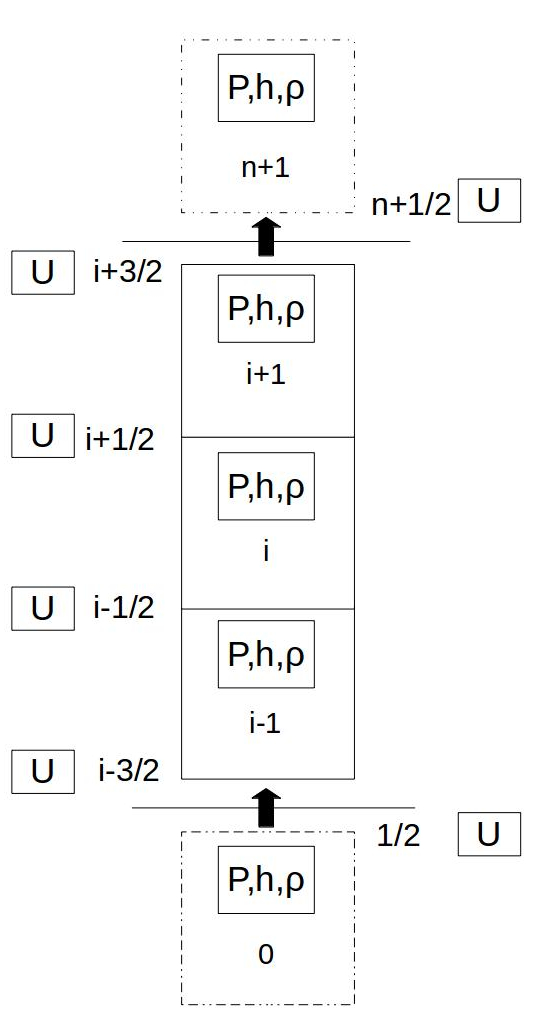
\includegraphics[width=0.30\textwidth]{images/CTF-Cells}
	\caption{The finite volume structure for COBRA-TF}
	\label{fig:CTF-Cells}
\end{figure}
    
\section{Sine Wave Advection Problem Setup}

The problem is to transiently vary the inlet enthalpy $h$ and inlet mass flow
rate $\dot{m}$ using a smooth trigonometric function so as to keep velocity
constant throughout the solution. Using a cosine, the analytical solution for a
variable $Y$ at time index $j$ and space index $i$, where $Y_{1}$ is the initial
value, $Y_{2}$ is the minimum value of the wave, and $P$ is the period of the
wave. The time step size $dt$, axial mesh size $dx$, and velocity $V_{o}$ are
assumed constant. If $V_{o}*j*dt>i*x$, then this equation doesn't apply and the
value should just equal the initial value $Y_{1}$.

\begin{equation}
	Y(i,j) = \frac{1}{2} \left( 
			(Y_{1}+Y_{2}) + (Y_{1}-Y_{2}) cos\left(
				\frac{2 \pi}{P} \left( j*dt + \frac{i*dx}{V_{o}} \right)
				\right)
			\right)
\end{equation}

This analytical solution can be applied to mass flow rate $\dot{m}$,
density $\rho$, liquid enthalpy $h$, and liquid temperature $T$. Since velocity
and pressure are cosntant, mass flow rate will be proportional to density, and
enthlapy will be proportional to temperature.

For the inlet condition, a transient data table was generated for enthalpy and
mass flow rate and applied at the inlet node. The comparison between the data
table and the output in CTF are shown for enthalpy and mass flow rate in figures
\ref{fig:Inlet_h} and \ref{fig:Inlet_m_dot} respectively. The CTF output was
read from hdf5 data files at each point in time, wich omitted the actual ghost
cell where these values were applied. The CTF values are located at the nearest
node to the inlet, and therefore will be slightly out of phase to the exact
values in the figure. This difference is more notable for smaller mesh sizes.

\begin{figure}[!h]
	\centering
	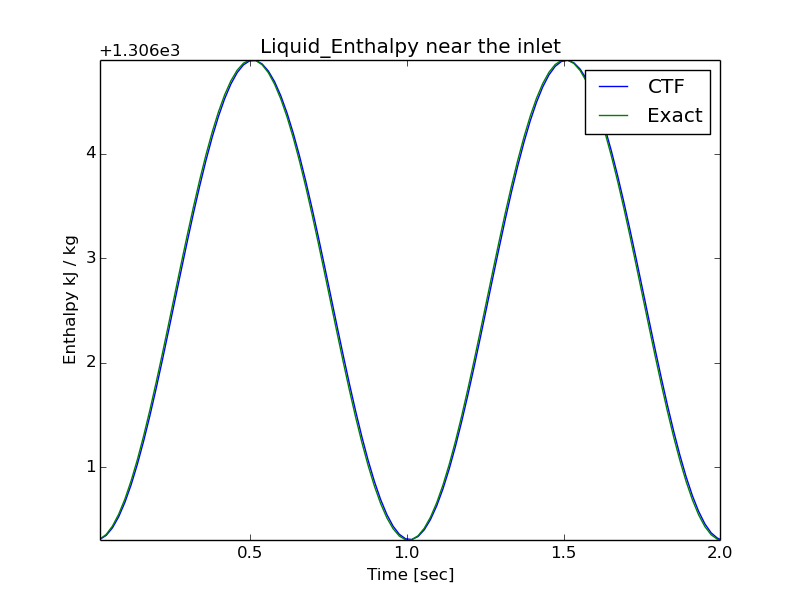
\includegraphics[width=0.675\textwidth]{images/Inlet_h}
	\caption{Enthalpy near the inlet and the analytical solution}
	\label{fig:Inlet_h}
\end{figure}

\begin{figure}[!h]
	\centering
	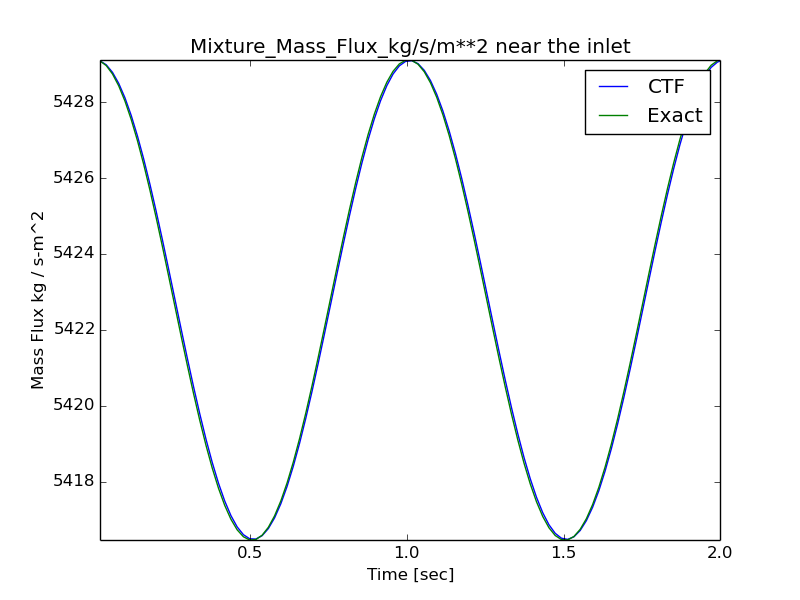
\includegraphics[width=0.675\textwidth]{images/Inlet_m_dot}
	\caption{Mass Flow rate near the inlet and the analytical solution}
	\label{fig:Inlet_m_dot}
\end{figure}

\section{Conclusions}

Present your summary and conclusions here.

%%%%%%%%%%%%%%%%%%%%%%%%%%%%%%%%%%%%%%%%%%%%%%%%%%%%%%%%%%%%%%%%%%%%%
\section{Acknowledgments}

Dr. Vince Mosseau, Dr. Maria Avramova, Dr. Kostadin Ivanov, and Nathan Porter.

%%%%%%%%%%%%%%%%%%%%%%%%%%%%%%%%%%%%%%%%%%%%%%%%%%%%%%%%%%%%%%%%%%%%%
\setlength{\baselineskip}{12pt}

\bibliographystyle{mc2015}
\bibliography{references}

%%%%%%%%%%%%%%%%%%%%%%%%%%%%%%%%%%%%%%%%%%%%%%%%%%%%%%%%%%%%%%%%%%%%%

%\appendix
%\section{}


\end{document}
